\chapter{Techno-Economic Analysis}

\section{Budget}
\label{appx:skripsie-budget}

\begin{table}[ht]
    \centering
    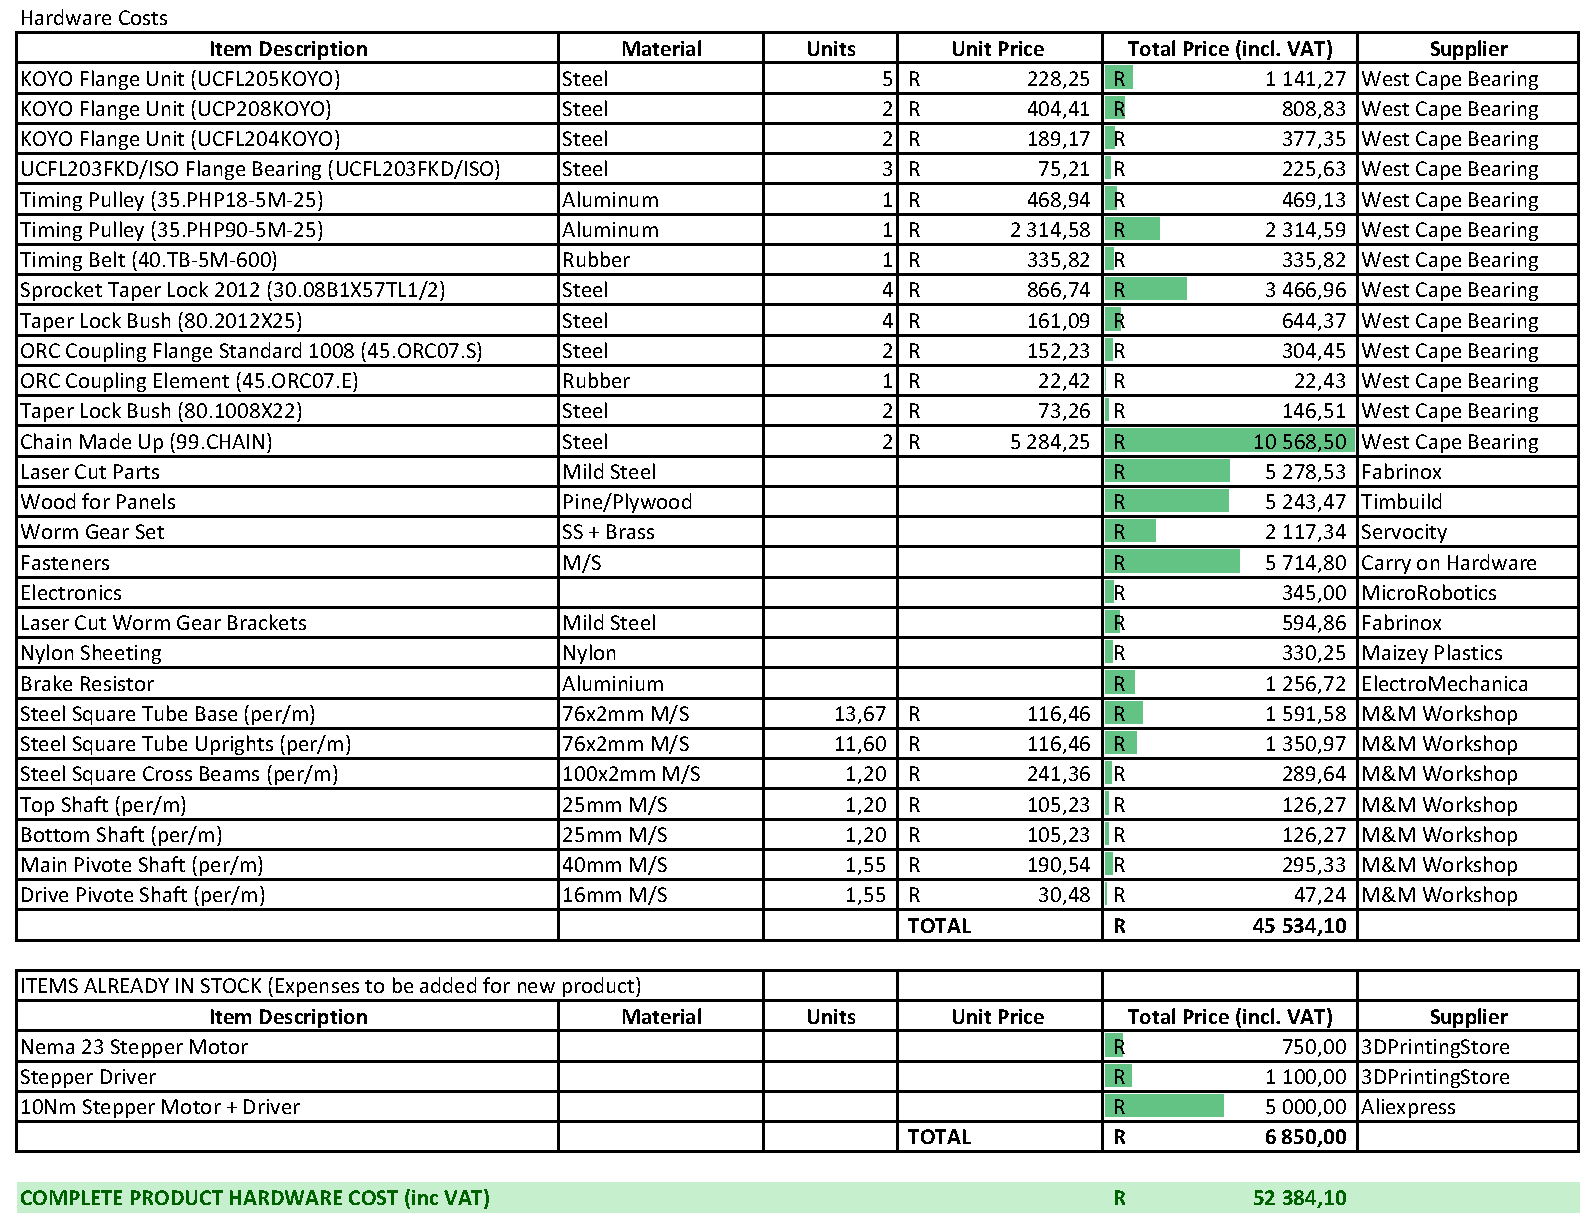
\includegraphics[width=1\linewidth]{tables/hardware_BOM.pdf}
    \caption{Hardware Bill of Materials}
    \label{tab:hardware-BOM}
\end{table}


\begin{table}[ht]
    \centering
    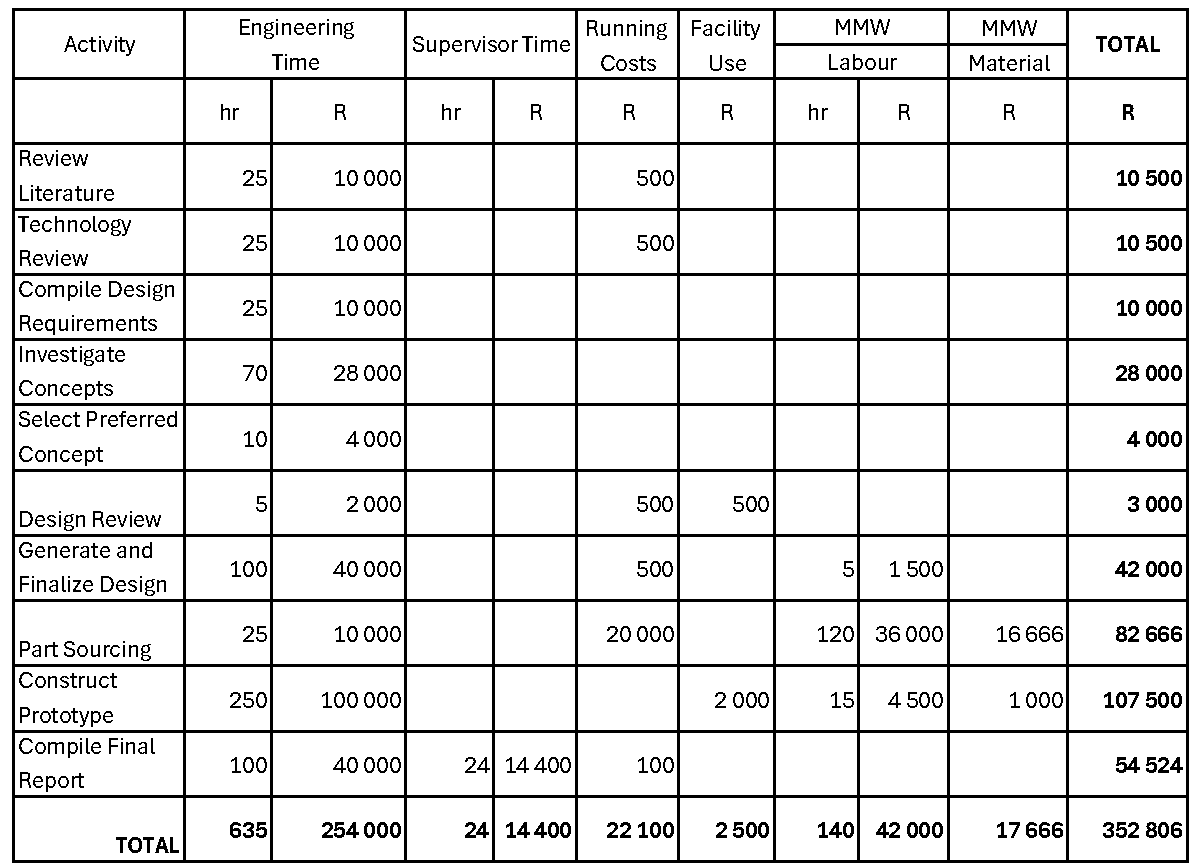
\includegraphics[width=1\linewidth]{tables/skripsie_budget_1.pdf}
    \caption{Proposed Skripsie Budget}
\end{table}

\begin{table}[ht]
    \centering
    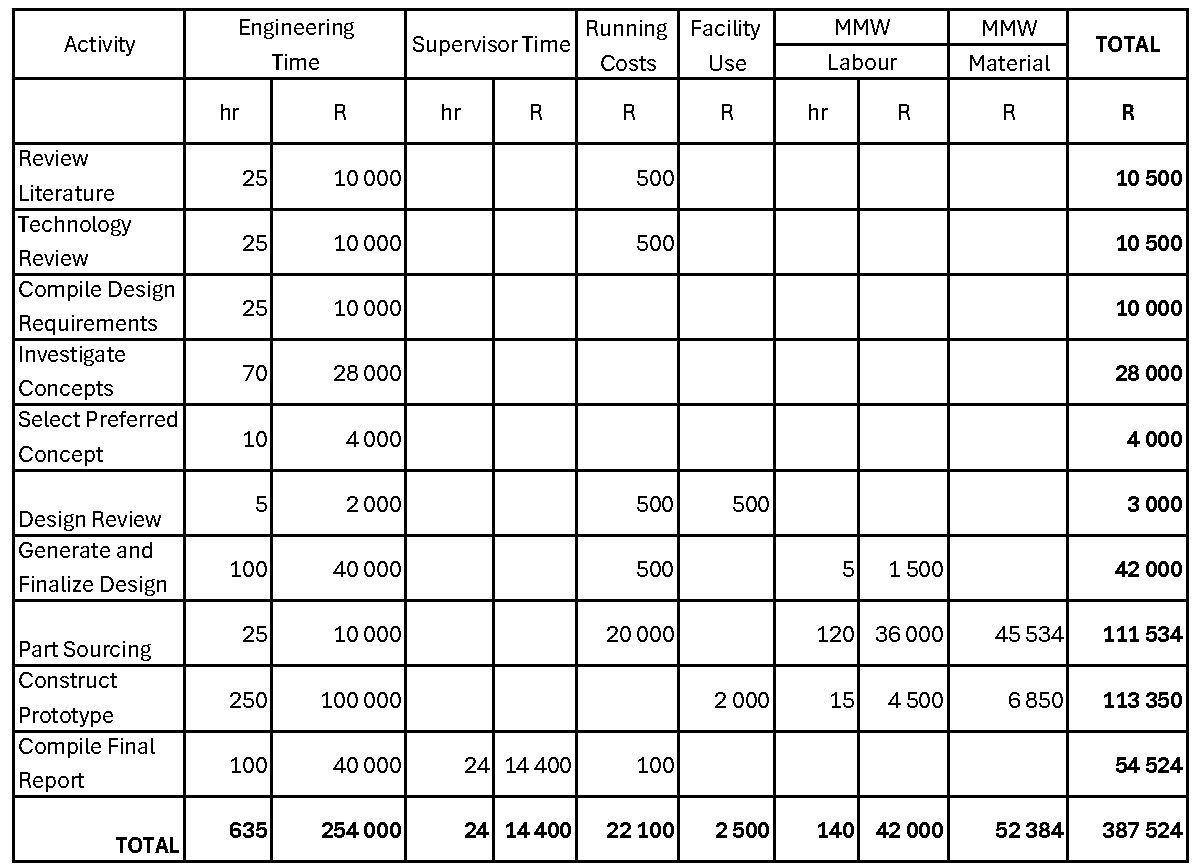
\includegraphics[width=1\linewidth]{tables/skripsie_budget_2.pdf}
    \caption{Realized Skripsie Budget}
\end{table}

\section{Time Management}

The project was completed on time, largely due to significant progress made during the June/July recess, focusing on research and finalizing the CAD design. This allowed the final drawing pack to be submitted to the workshop in the first week of the second semester, enabling fabrication to begin promptly. Some minor delays occurred during the manufacturing phase, mainly due to material sourcing and small design adjustments, which caused a slight postponement in the construction timeline. The Gantt chart depicting the project's progress is shown in Figure \ref{fig:gantt_final}.

\begin{figure}[ht]
    \centering
    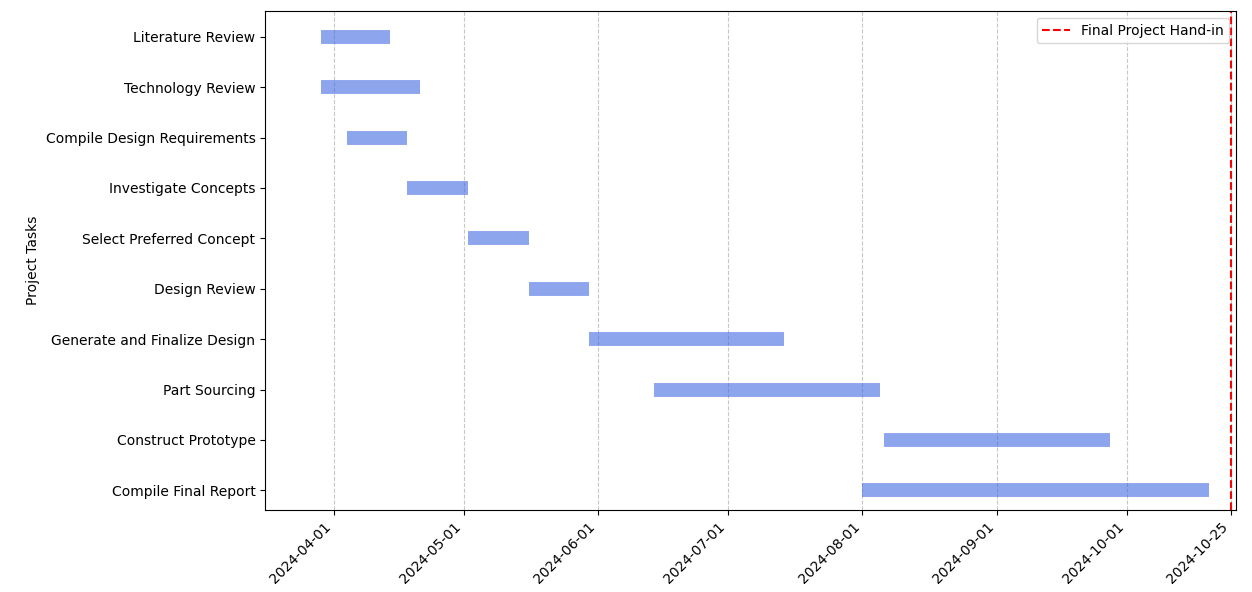
\includegraphics[width=1\linewidth]{figs/gantt_final.png}
    \caption{Gantt chart showing project timeline}
    \label{fig:gantt_final}
\end{figure}

\chapter{Responsible Use of Resources and End-of-Life Strategy}

Responsible resource use was a key consideration from the outset of the design process. Designs and drawings were thoroughly checked for accuracy to minimize waste from iterations, redesigns, or remanufacturing. Appropriate calculations and simulations were conducted to reduce the need for redesign. Where possible, low-impact materials were selected. For instance, standard, readily available, and low-cost steel tubing and shafts were used for the frame, while wood was chosen for the panels, which can be reused if needed, rather than opting for specialized materials.

In an effort to avoid waste, the system will be commissioned for long-term use, as it will be sold to a private buyer for personal use, ensuring its continued functionality. If the system is decommissioned in the future, most of the steel components can be disassembled and returned to the workshop for reuse in future projects, as very few parts were machined in a way that would prevent them from being repurposed. The wooden components can also be reused, and any parts that cannot be reused will be recycled where possible.
